\documentclass{article}
\usepackage[T1]{fontenc}
\usepackage{lmodern}
\usepackage{graphicx}
\usepackage{amsmath,amssymb}
\usepackage[a4paper,margin=2cm]{geometry}
\usepackage[absolute,overlay]{textpos}
\setlength{\TPHorizModule}{1mm}
\setlength{\TPVertModule}{1mm}
\usepackage[indonesian]{babel}
\usepackage{hyperref}
\setlength{\emergencystretch}{2em}
% unit: Halaman 15

\begin{document}

% === Halaman 15 (python/native) ===

Rinaldi M/II4020 Kriptografi

15

Contoh: Alice dan Bob menyepakati  p = 353 dan g = 3  ( 3 < 353, dan 3 adalah akar primitif 353)

1.

Alice memilih a = 97 dan menghitung


    A = ga mod p = 397 mod 353 = 40


Alice mengirim A kepada Bob.

2.

Bob memilih b = 233 dan menghitung


    B = gb mod p = 3233 mod 353 = 248


Bob mengirim B kepada Alice.

3.

Alice menghitung kunci rahasia K,



 K = Ba mod p = 24897 mod 353 = 160

4.

Bob menghitung kunci rahasia K,



 K = Ab mod p = 40233 mod 353 = 160

Jadi, Alice dan Bob sekarang sudah mempunyai kunci  rahasia yang sama, yaitu K = 160. Mereka 

dapat menggunakan K sebagai kunci enkripsi dan dekripsi pesan dengan algoritma kunci simetri.

% deskripsi: gambar native xref 75
\noindent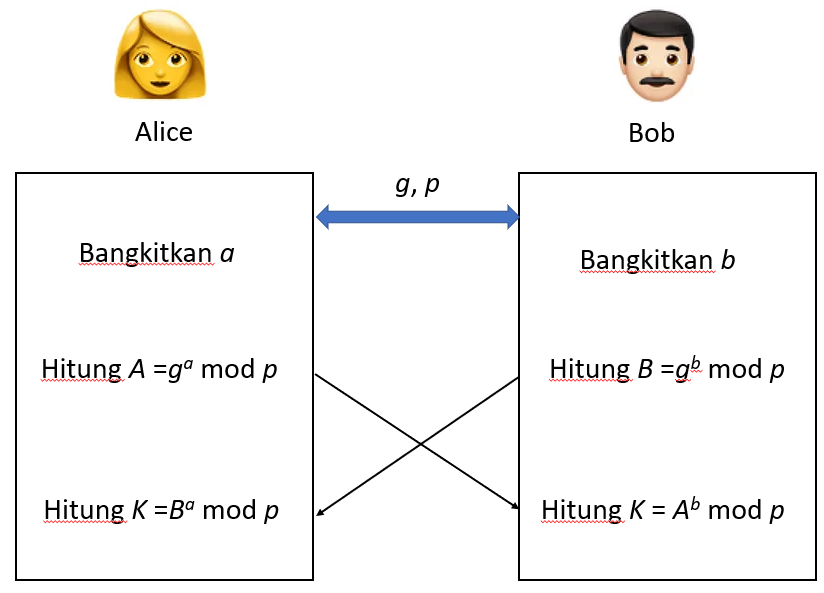
\includegraphics[width=0.85\textwidth]{../../images/python/page_015_img_01.png}

\end{document}
